\chapter{Frame Synchronization} \label{ch:Frame_sync}

Frame synchronization is a well-known problem in the literature. We receive several frames with a defined length and a preamble (ASM) designed to locate them. To search for the preamble within the received samples and thus locate each frame, there are two techniques mentioned in the standard \autocite{CCSDS_130_1_G_3}:

First, an intuitive approach would be to search for the decoded preamble using the $\mathtt{Viterbi}$ algorithm. Since the ASM is a pseudorandom code specified in \autocite{CCSDS_131_0_B_5}, it could be correlated\footnote{Although there are other methods to find a known bit string, the correlation method has been chosen and is widely used in the literature.} with the preamble until it is found. However, we face the problem of the phase ambiguity of the Costas loop; the constellation after the block can appear rotated. 

Secondly, it is possible to correlate with the preamble before synchronization and the $\mathtt{Viterbi}$ decoder by searching for the sequence encoded by the convolutional code. Although the output of the convolutional code depends on the previous $K$ bits, and assuming that those bits are random, once we bypass those bits, the encoder output will yield the same result if the input is the same. If the ASM preamble measures $32$ bits, then the preamble encoded with a rate $1/2$ CC will measure $64$ bits, of which $50$ bits will be identical\footnote{As a curiosity, the standard is very rigorous regarding spurious signals and power peaks at certain frequencies. By having $50$ repeating bits, spectral peaks will be generated at a distance of frame\_length / (frame\_length + ASM)*Ts. Since these bits have a very low power compared to the other bits that make up the frame, this is considered permissible.} since $K=7$ (Remember \Cref{sec:cc}). 

\begin{figure}[h]
    \centering
    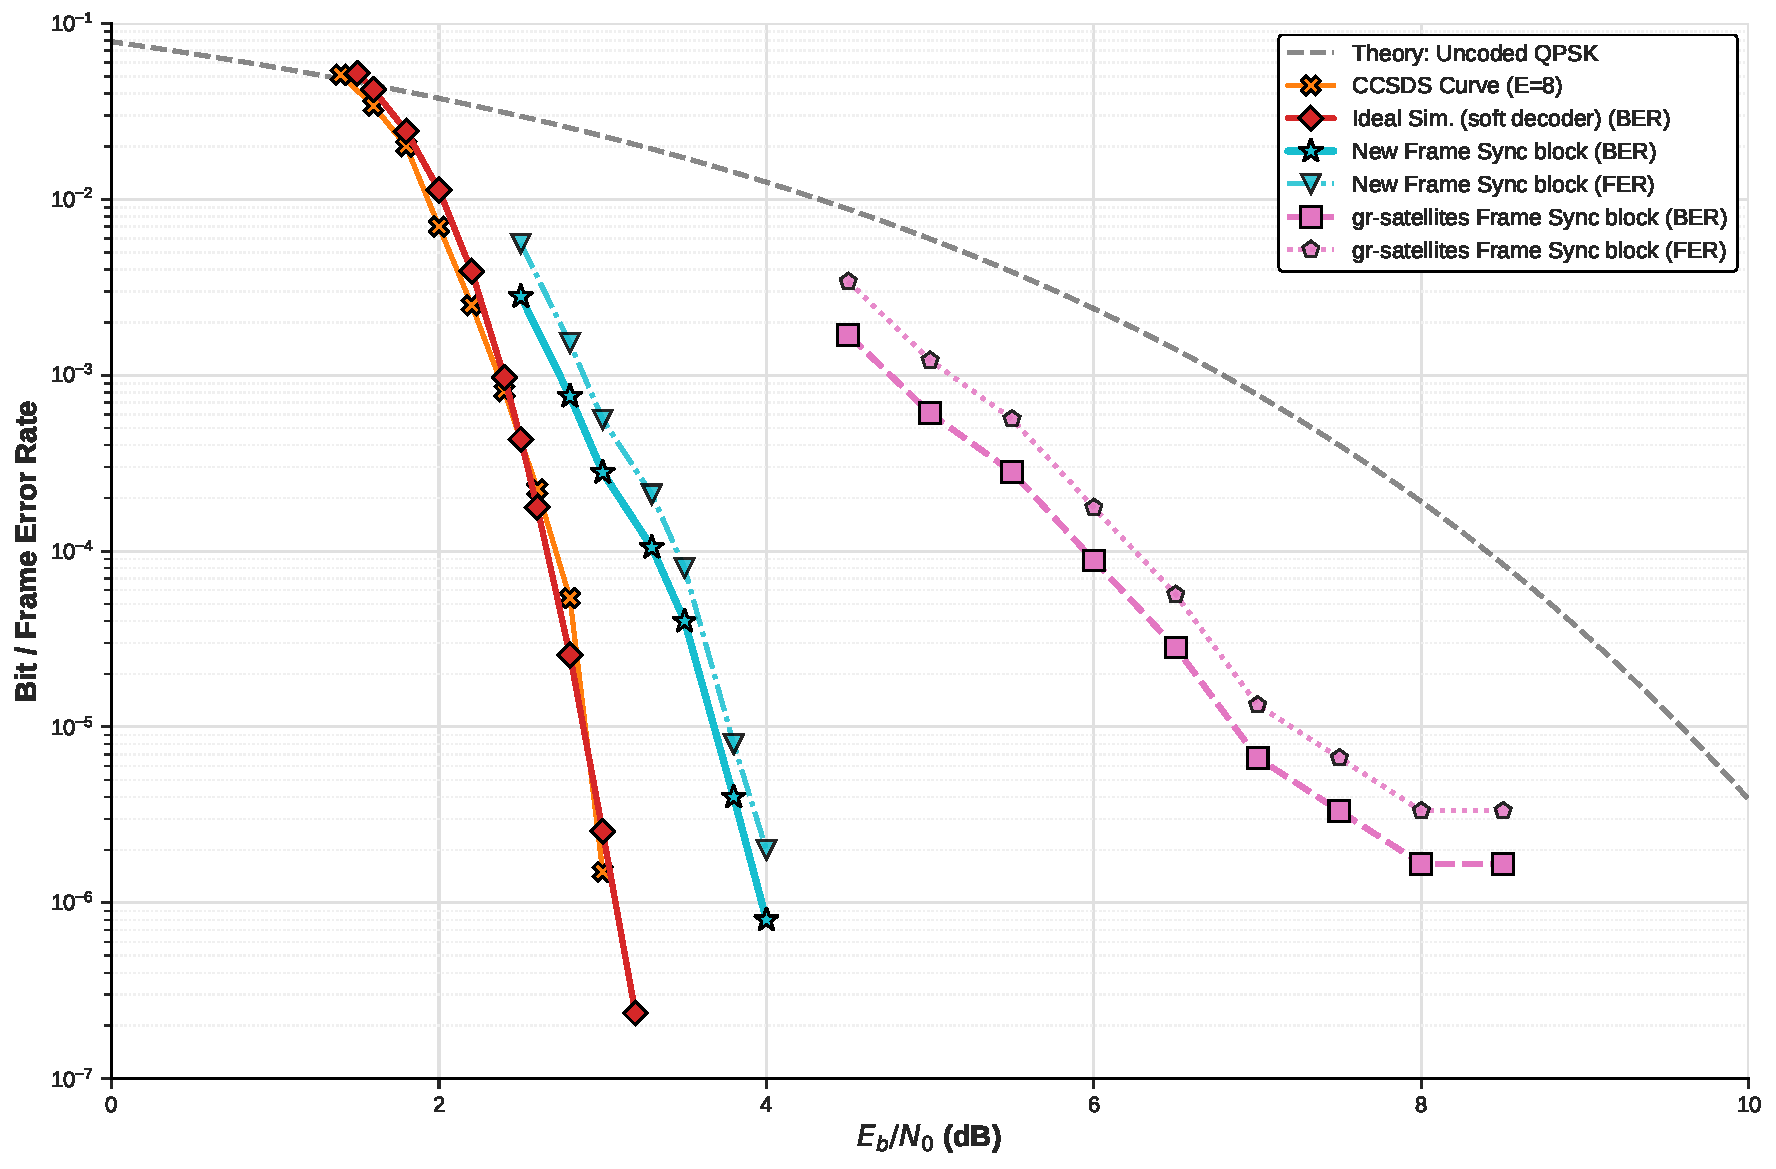
\includegraphics[width=1\textwidth]{figures/Inkscape/BER_curves_frame_sync1.pdf}
    \caption{Performance comparison between the standard frame synchronization algorithm provided by the \texttt{gr-satellites} library and a custom-implemented synchronizer.}
    \label{fig:BER_curves_frame_sync}
\end{figure}

Although it may seem that searching for $50$ bits is better than searching for $32$ --- even though the coding gain is a factor to consider ---, those bits are being searched for without having fine frequency synchronization. Therefore, a search based on some differential scheme is necessary. An advantage offered here is resolving the phase ambiguity problem, since the GNU Radio Costas loop implementation accepts a tag indicating the relative phase, which can be obtained by correlating.

In this report, we have focused on implementing the first solution.


\section{Algorithms Already Implemented in GNU Radio}

Several blocks that implement very similar algorithms to solve this problem can be found online. In general, they all focus on correlating with the preamble, and if the result of the correlation is greater than an established value (threshold), then a metadata tag is added and it is considered that the preamble (and consequently the frame) has been found. In the GNU Radio implementations \href{https://wiki.gnuradio.org/index.php/Correlation_Estimator}{\texttt{Correlation Estimator}} and in the gr-satellites library \href{https://github.com/daniestevez/gr-satellites/blob/main/python/components/deframers/ccsds_rs_deframer.py}{\texttt{CCSDS Deframer}}, the correlation is performed against the entire incoming bit block, generating false negatives and false positives, which drastically reduces the viability of the link at low \(\mathsf{SNR}\).

\begin{figure}[h]
    \centering
    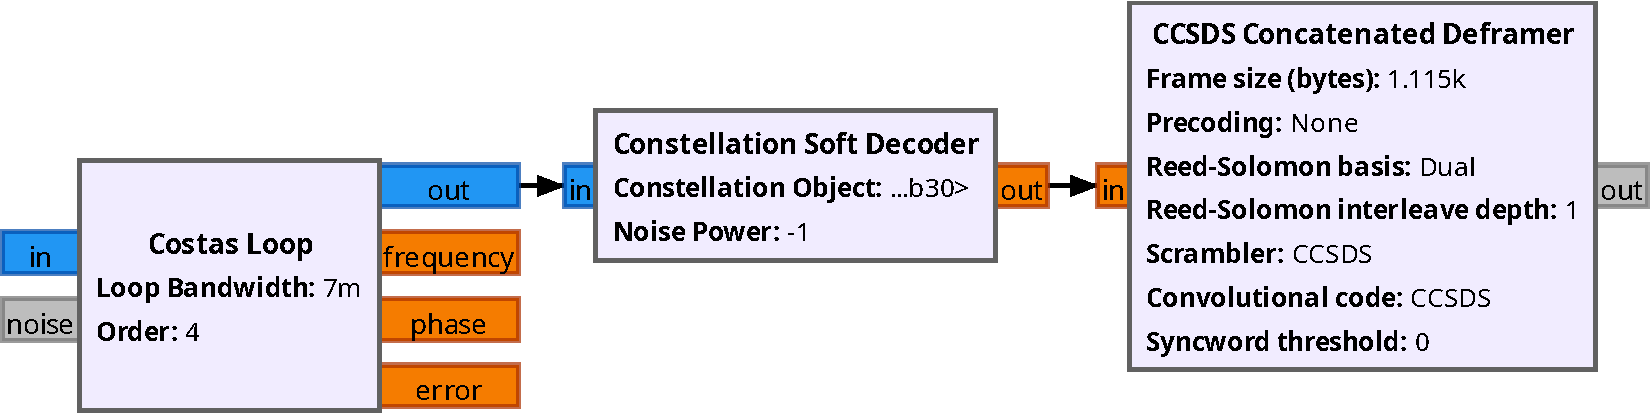
\includegraphics[width=0.65\textwidth]{figures/Inkscape/frame_sync.pdf} 
    \caption{Receiver architecture with the deframer block from \autocite{gr_satellites} library.}
    \label{fig:already_frame_sync} 
\end{figure}

To understand the limits of using an Access Sync Marker (ASM) of length $N=32$ with an error threshold $T=3$ (we tolerate up to 3 bits of difference), we must separate the channel's physical Bit Error Rate ($p$) from the correlator's False Alarm Probability ($P_{FA}$). While $T=3$ ensures robust synchronization in noisy channels (tolerating up to $p \le 0.026$), continuously correlating the entire incoming bitstream introduces a major issue: false positives.

Assuming the payload or ambient noise acts as random data ($p_{rand} = 0.5$), the probability of a random sequence falsely matching the ASM within our 3-bit tolerance is:
\begin{equation}
    P_{FA} = \sum_{k=0}^{3} \binom{32}{k} (0.5)^{32} \approx 1.28 \times 10^{-6}
\end{equation}
Consequently, $T=3$ creates an artificial error floor. Even if the radio link is perfect (infinite SNR with zero physical errors), the receiver will still trigger a false sync approximately once every $7.8 \times 10^5$ bits. Since the system's effective error rate can never drop below this $1.28 \times 10^{-6}$ limit, relying on continuous brute-force correlation is suboptimal. You can see in \Cref{fig:BER_curves_frame_sync} the fictitious floor in the pink curve. The algorithm must be improved, for example, by implementing a state machine that only opens correlation windows where the next preamble is actually expected, as the standard says.

\subsection{Phase Ambiguity}

In fact, the phase ambiguity problem is not completely resolved. Since QPSK is used, we have an unknown phase at the output of the Costas loop. The constellation may have rotated $0$, $\pi/2$, $\pi$, or $3\pi/2$ radians depending on which quadrant the Costas loop managed to lock onto after an assumed loss of lock. 

On the other hand, we have a $\mathtt{Viterbi}$ decoder which is transparent, meaning that if the input to the $\mathtt{Viterbi}$ is inverted (assume the case of a $\pi$ radians ambiguity), then the output will also be inverted. This allows applying the algorithms by searching for the phase $0$ ASM and the \invASM~rotated by $\pi$ radians. This is, in fact, what is already implemented in gr-satellites \href{https://github.com/daniestevez/gr-satellites/blob/main/python/components/deframers/ccsds_concatenated_deframer.py}{\texttt{Concatenated Deframer}}. However, what happens when the phase ambiguity is $\pi/2$ or $3\pi/2$? The $\mathtt{Viterbi}$ decoder is unable to decode and outputs garbage. This latter issue is not addressed in the found implementations since they are mainly based on BPSK (therefore, the constellation can only be rotated by $\pi$ radians, and since the decoder is transparent, there is no problem). 

Finally, the standard \autocite[Section 9.3.7]{CCSDS_130_1_G_3} recommends applying a multi-state flywheel algorithm. In this way, once a frame is found ("search" state), the algorithm transitions to a "lock" state and considers that there are up to a configurable number $N$ of frames in the space adjacent to the found frame, even if the ASM has not been found. This allows recovering the frame even if the preamble has been destroyed by an error burst and we solve the problem of false positives that we were talking about.

\begin{figure}[h]
    \centering
    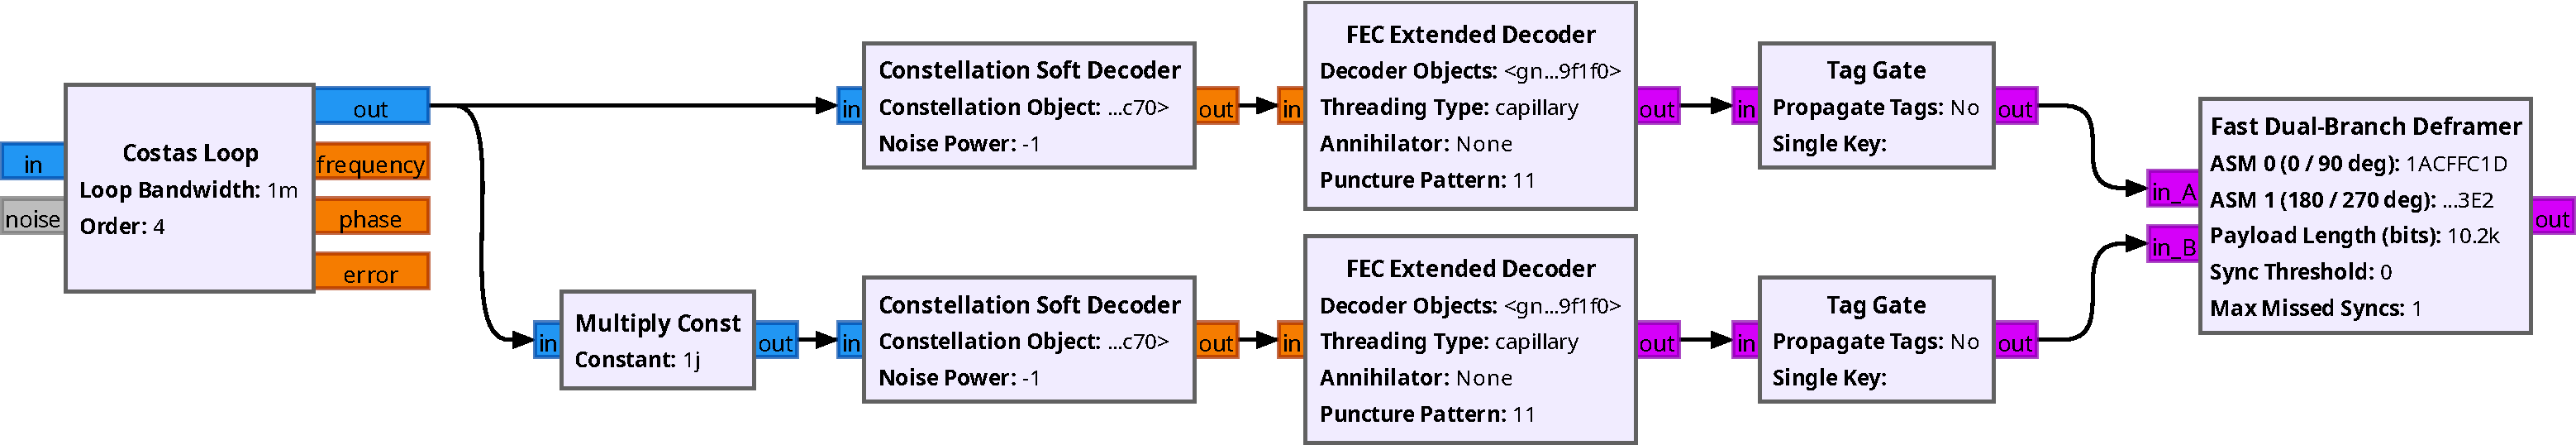
\includegraphics[width=1\textwidth]{figures/Inkscape/flywheel2.pdf} 
    \caption{Dual-branch receiver architecture with parallel Viterbi decoding and fast synchronization.}
    \label{fig:flywheel_blocks} 
\end{figure}


\section{Solving the Phase Problem}

Having outlined the phase ambiguity problem introduced by the Costas loop (which can lock at $0$, $\pi/2$, $\pi$, or $3\pi/2$ radians) and the limitations of existing implementations, it is necessary to implement a custom, robust synchronization algorithm. 

While a brute-force approach running four parallel decoding pipelines is computationally feasible on modern hardware, a more resource-efficient trade-off can be achieved. Because the $\mathtt{Viterbi}$ decoder is transparent to $\pi$-radian phase inversions, the ambiguity can be fully resolved using only two parallel branches. The first branch processes the incoming soft symbols directly (covering the $0$ and $\pi$ shifts), while the second branch processes a $\pi/2$-rotated version of the symbols (covering the $\pi/2$ and $3\pi/2$ shifts).

An initial feedback-based approach using asynchronous messages to rotate the Costas loop output was evaluated. However, this design was discarded because buffer latencies caused a systematic loss of frames during phase slips (a detailed analysis of this discarded architecture and its state machine is provided in \ref{app:async_sync}). 

\begin{figure}[h]
    \centering
    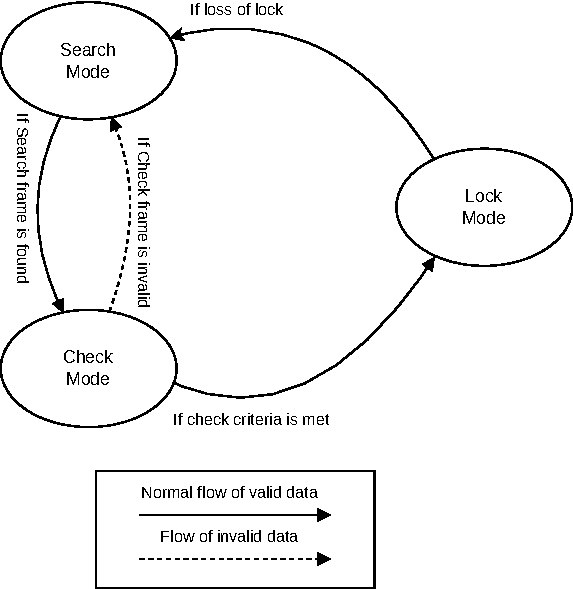
\includegraphics[width=0.5\textwidth]{figures/Inkscape/states2.pdf} 
    \caption{Three-state diagram (Search/Lock) for the dual-branch frame synchronizer.}
    \label{fig:states} 
\end{figure}

To achieve zero-latency recovery and eliminate frame loss, the custom dual-branch synchronizer employs a highly optimized three-state machine (see \Cref{fig:states}) that operates continuously on both data streams:

\begin{itemize}
    \item \textcolor{gray}{Search mode}: The $32$-bit ASM and its inverted version are simultaneously searched across both the standard and the $\pi/2$-rotated branches. Upon detecting a candidate synchronization marker within the acceptable bit-error threshold, the algorithm transitions to \textit{Check} mode.
    \item \textcolor{gray}{Check mode}: In this intermediate verification state, the algorithm evaluates the synchronization criteria to ensure the detected marker is not a false positive generated by random payload data. It confirms the validity of the sequence, definitively selects the active branch containing the valid data stream, and transitions to \textit{Lock} mode.
    \item \textcolor{gray}{Lock mode}: The search window systematically jumps forward by the exact frame length to evaluate the subsequent ASM on the active branch (flywheel operation). If the ASM is missing or corrupted beyond the threshold, a \texttt{max\_misses} counter is incremented. If this counter overflows—indicating a genuine loss of synchronization or a Costas loop phase slip—the system instantly drops the current branch and returns to \textit{Search} mode. Because the alternative branch is already being decoded in parallel, the synchronizer can re-establish lock on a new phase almost instantaneously.
\end{itemize}


\section{Results}

By leveraging this dual-branch feed-forward architecture, the receiver maintains precise synchronization regardless of the Costas loop's phase orientation. Since both the non-rotated and $\pi/2$-rotated symbols are continuously fed into parallel $\mathtt{Viterbi}$ decoders, a phase slip simply triggers a rapid transition from \textit{Lock} to \textit{Search} mode, where the algorithm instantly latches onto the alternative branch. 

The improvements in link viability are clearly demonstrated in \Cref{fig:BER_curves_frame_sync}. The Bit / Frame Error Rate is plotted against the $E_{b}/N_{0}$ (dB). As previously theorized, the continuous brute-force correlation used by the gr-satellites Frame Sync block (BER) and the gr-satellites Frame Sync block (FER) creates an artificial error floor, preventing the error rate from dropping below the $10^{-6}$ limit. In contrast, the New Frame Sync block (BER) closely tracks the Ideal Sim. (soft decoder) (BER) curve without exhibiting any artificial floor. By actively gating the correlation windows through the three-state machine, the new synchronizer avoids false alarms from payload data or ambient noise, ensuring near-ideal performance.


\begin{comment}
    
\section{Solving the Phase Problem}

Having outlined the phase ambiguity problem and the limitations of the found implementations, I find it necessary to implement a custom algorithm to solve these issues. There are two strategies:

In the first instance, based on some implementations found in examples within the GNU Radio community, it is common to place $4$ parallel branches at the output of the soft decisions block and rotate each one in order to search for the four possible phases at the output of the Costas loop. Each branch must be rotated, passed through the $\mathtt{Viterbi}$ decoder, and additionally perform the correlation to find the preamble. A coherent result will be found in only one of those $4$ branches, and only one branch will pass to the subsequent blocks. Using a sledgehammer to crack a nut might work well, but it's not the best option if my resources are limited. See the chapter \Cref{ch:Link} where optimization and resource consumption are discussed further. 

\begin{figure}[h]
    \centering
    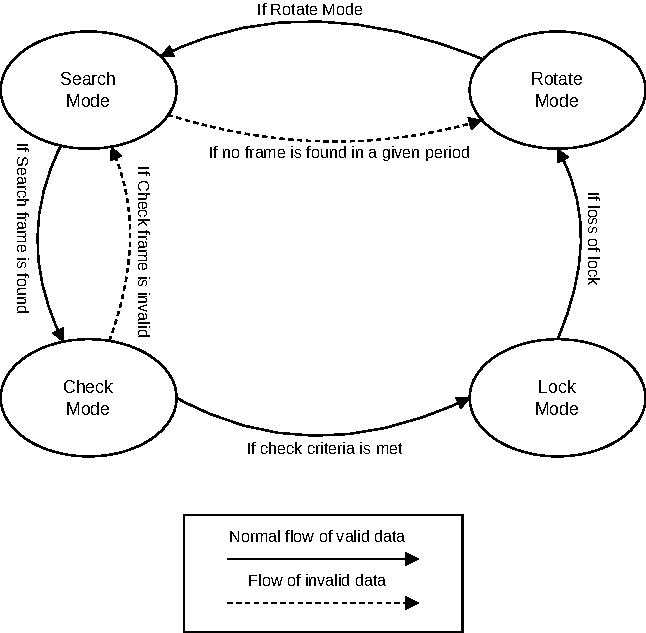
\includegraphics[width=0.65\textwidth]{figures/Inkscape/states.pdf} 
    \caption{States diagram of the flywheel algorithm for frame synchronization.}
    \label{fig:states} 
\end{figure}

On the other hand, the idea occurred to me to add another `rotation" state where, if the ASM is not found, it is assumed that the constellation has rotated, and an asynchronous message is sent to a block placed after the Costas loop whose function is to rotate the phase by $\pi$ radians. Thus, assuming that the Costas loop genuinely rotated the constellation, the problem would disappear if the unrotated version and the $\pi$-radians rotated version of the preamble are searched simultaneously (remember that the decoder is transparent). This algorithm is depicted in the state diagram \Cref{fig:states}.

\begin{itemize}
    \item \textcolor{gray}{Search mode}: The $32$-bit preamble is searched for within the received bits. If the preamble detects what appears to be the start of a frame, it transitions to the \textit{check} mode. If the preamble is not detected within a certain time, it switches to the \textit{rotate} mode.
    \item \textcolor{gray}{Check mode}: It verifies that the detected bits pass the criteria.
    \item \textcolor{gray}{Lock mode}: The search window jumps a space equal to the frame length and checks for the preamble. In case it is not found, the \texttt{max\_misses} variable is incremented by one. If the \texttt{max\_misses} variable overflows, then it assumes the phase has changed and sends a message to activate the \textit{rotate} mode.
    \item \textcolor{gray}{Rotate mode}: If the message is received, the \textit{rotate} mode (implemented in a different block from the other modes) rotates the constellation by $90^\circ$. Afterwards, it returns to the \textit{search} mode.
\end{itemize}



Upon implementing the algorithm and programming it in C++, we got much closer to the standard curves, thereby improving the viability of the link. Look at the figure \autocite[figure]{CCSDS_401_0_B_32} where the curve obtained with the algorithm is plotted against the curve we obtained with the blocks found on the web.

\section{Results}

Despite having provided a solution to the phase ambiguity problem, this implementation brings with it a disadvantage: every time the Costas loop causes a phase change, $5$ frames are lost. As we have well mentioned, the message to rotate the constellation is asynchronous. Imagine that we are in the ``Lock" state, the constellation rotates, and the lock mode assumes that there is a frame in the next space even though it has not found the preamble. The \texttt{max\_misses} variable that controls the state change to `Rotate" is incremented by one. The next frame arrives, the preamble is also not found; if \texttt{max\_misses} is set to $1$, then here it overflows and changes to the `Rotate" state. The asynchronous message is sent to the rotation block, which rotates the phase by $90^\circ$. At that instant, there is already one frame being processed in the $\mathtt{Viterbi}$ decoder, one frame in the $\mathtt{Viterbi}$ output buffer, and another frame in the input buffer of the synchronization algorithm. In total, we lose $5$ frames. 

\begin{figure}[h]
    \centering
    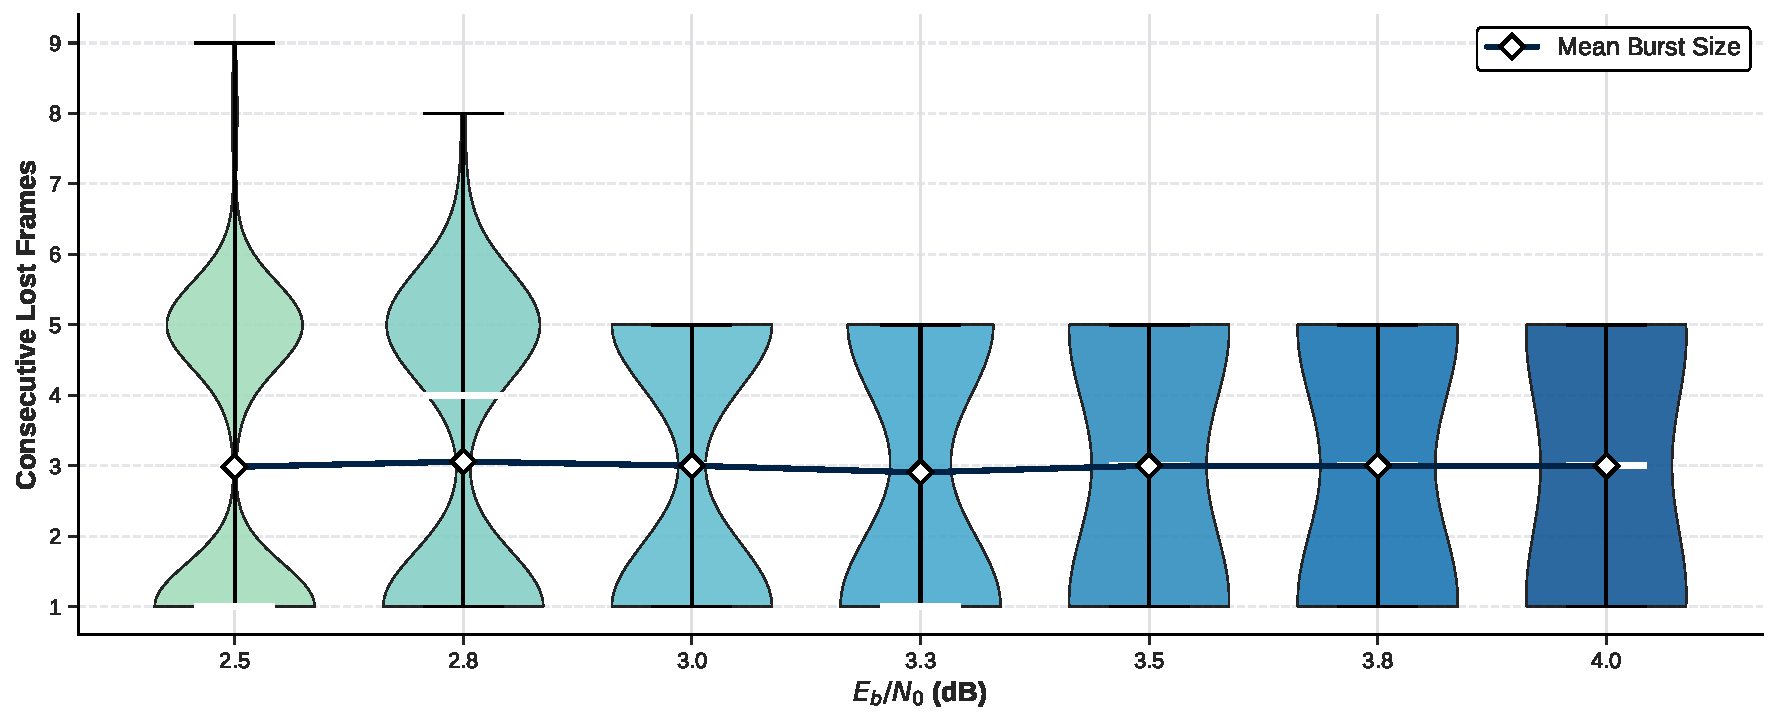
\includegraphics[width=0.8\textwidth]{figures/Inkscape/Doppler_BurstLoss.pdf} 
    \caption{Distribution of Sync Loss Burst Sizes (Doppler Soft 5m)}
    \label{fig:Comparative_frame_sync}
\end{figure}

In this case, it seems like a good idea to reduce \texttt{max\_misses} to $0$, since we would lose $4$ frames instead of $5$ every time the Costas loop rotates the phase. However, it has been observed experimentally that finding $1$ erroneous bit within the $32$ bits of the ASM is more probable than the Costas loop losing lock. The difference becomes evident at a higher $E_b/N_0$ since the Costas loop always remains locked. \Cref{fig:Comparative_frame_sync} is generated with \texttt{max\_misses} set to 1, providing optimal results relative to the received power analyzed in \Cref{ch:Link}.







\end{comment}